\centerline{\bf \huge 9 класс}
\centerline{\normalsize{\it Работа рассчитана на \bf{180} минут}}

\problem{9.1}
Найдите наибольшее пятизначное число, произведение цифр которого равно 120.

\textit{Ответ: 85311.}

\textit{Решение.} Наибольший однозначный делитель числа $120-8$, поэтому искомое число точно начинается с этой цифры. Произведение всех оставшихся цифр равняется 15.

Наибольший однозначный делитель числа $15-5$, поэтому в разряде тысяч будет стоять именно эта цифра. Произведение последних трёх цифр равняется трём 3, поэтому наибольшее число будет заканчиваться на 311.

\problem{9.2}
Лентяйка Эвена жёстко готовится к муниципу по математике. Чтобы не растратить все силы, она решает не более 10 задач в день, а если в какой-нибудь день она решала больше 7 задач, то следующие два дня она решала не более 5 задач в день. Какое наибольшее количество задач Эвена могла решить за 7 подряд идущих дней?

\textit{Ответ: 52.}

\textit{Решение.}
Предположим, Эвена решила в один из первых пяти дней хотя бы 8 задач (но не больше 10), тогда в следующие два дня она решала не более 5 задач в день. Таким образом, за эти три дня она решила не более $20(10+5+5)$ задач. Если бы она в каждый из этих дней решала по 7 задач, то вышло бы больше.

Получается, в первые пять дней Эвена решила не более 35 задач. Осталось заметить, что в последние два дня она решила не более 17 задач (так как она не могла в оба дня превысить порог в 7 задач), при этом 17 задач она решить могла (7 задач в шестой день и 10 задач в седьмой день).

\problem{9.3}
Про положительные числа $a, b, c$ известно, что

$$
\frac{a+b+c}{a+b-c}=7, \quad \frac{a+b+c}{a+c-b}=1,75 .
$$


Чему равняется $\frac{a+b+c}{b+c-a}$ ?

\textit{Ответ: 3,5.}

\textit{Решение.}
Пусть $\frac{a+b+c}{b+c-a}=x$. Заметим, что

$$
\begin{gathered}
\frac{1}{7}+\frac{1}{1,75}+\frac{1}{x}=\frac{a+b-c}{a+b+c}+\frac{a+c-b}{a+b+c}+\frac{b+c-a}{a+b+c}=1 \\
\frac{1}{7}+\frac{4}{7}+\frac{1}{x}=1 \\
x=3,5
\end{gathered}
$$


%все задачи выше муницип Москва 2020

\problem{9.4}
Алина и Маша разложили на столе 13 различных карт. Каждая карта может лежать в одном из двух положений: рубашкой вверх или рубашкой вниз. Игроки должны по очереди переворачивать по одной карте. Проигрывает тот игрок, после хода которого повторится какая-то из предыдущих ситуаций (включая изначальную). Первый ход сделала Маша. Кто сможет выиграть независимо от того, как будет играть соперник?

\textit{Решение.}
Выигрышная стратегия Маши состоит в том, чтобы каждый раз переворачивать одну и ту же карту (например, пиковую даму). Все возможные позиции можно разбить на пары, отличающиеся лишь расположением пиковой дамы. Если в ответ на ход Маши Алина тоже перевернёт пиковую даму, то повторится предыдущая позиция, и она проиграет. Поэтому она вынуждена переворачивать другую карту. А Маша, перевернув в ответ пиковую даму, получит позицию, парную к той, которая только что была. Таким образом, каждым ходом Алине придётся <<начинать>> новую пару, и Маша всегда сможет сделать ответный ход, <<закончив>> пару. Так как количество возможных позиций конечно, то рано или поздно Алина не сможет открыть новую пару и проиграет.
%Москва 2016

\problem{9.5}
В остроугольном треугольнике $A B C$ проведена медиана $B M$. Точки $P$ и $Q$ --- центры вписанных окружностей треугольников $A B M$ и $C B M$ соответственно. Докажите, что вторая точка пересечения описанных окружностей треугольников $A B P$ и $C B Q$ лежит на отрезке $B M$.

\textit{Решение.}
Отметим на $B M$ точку $D$ так, что $M A=M D=M C$. Так как $\angle A B C<\angle A D C=90^{\circ}$, то эта точка лежит на отрезке $B M$ (см. рис. 1). Докажем, что описанные окружности треугольников $A B P$ и $C B Q$ вторично пересекаются в точке $D$.

Действительно, пусть $\angle B M A=\varphi$.
Тогда $\angle B P A=90^{\circ}+\frac{\varphi}{2}$, так как он образован биссектрисами треугольника $A B M$. С другой стороны, из равнобедренного треугольника $A M D$ получим: $\angle A=\angle D=\frac{180^{\circ}-\varphi}{2}=90^{\circ}-\frac{\varphi}{2}$, тогда $\angle B D A=90^{\circ}+\frac{\varphi}{2}$. Равенство углов $B P A$ и $B D A$ означает, что описанная окружность треугольника $A B P$ проходит через $D$. Аналогично доказывается, что через $D$ проходит описанная окружность треугольника $C B Q$. Таким образом, эти окружности пересекаются на медиане $B M$, что и требовалось доказать.

\begin{figure}
    \centering
    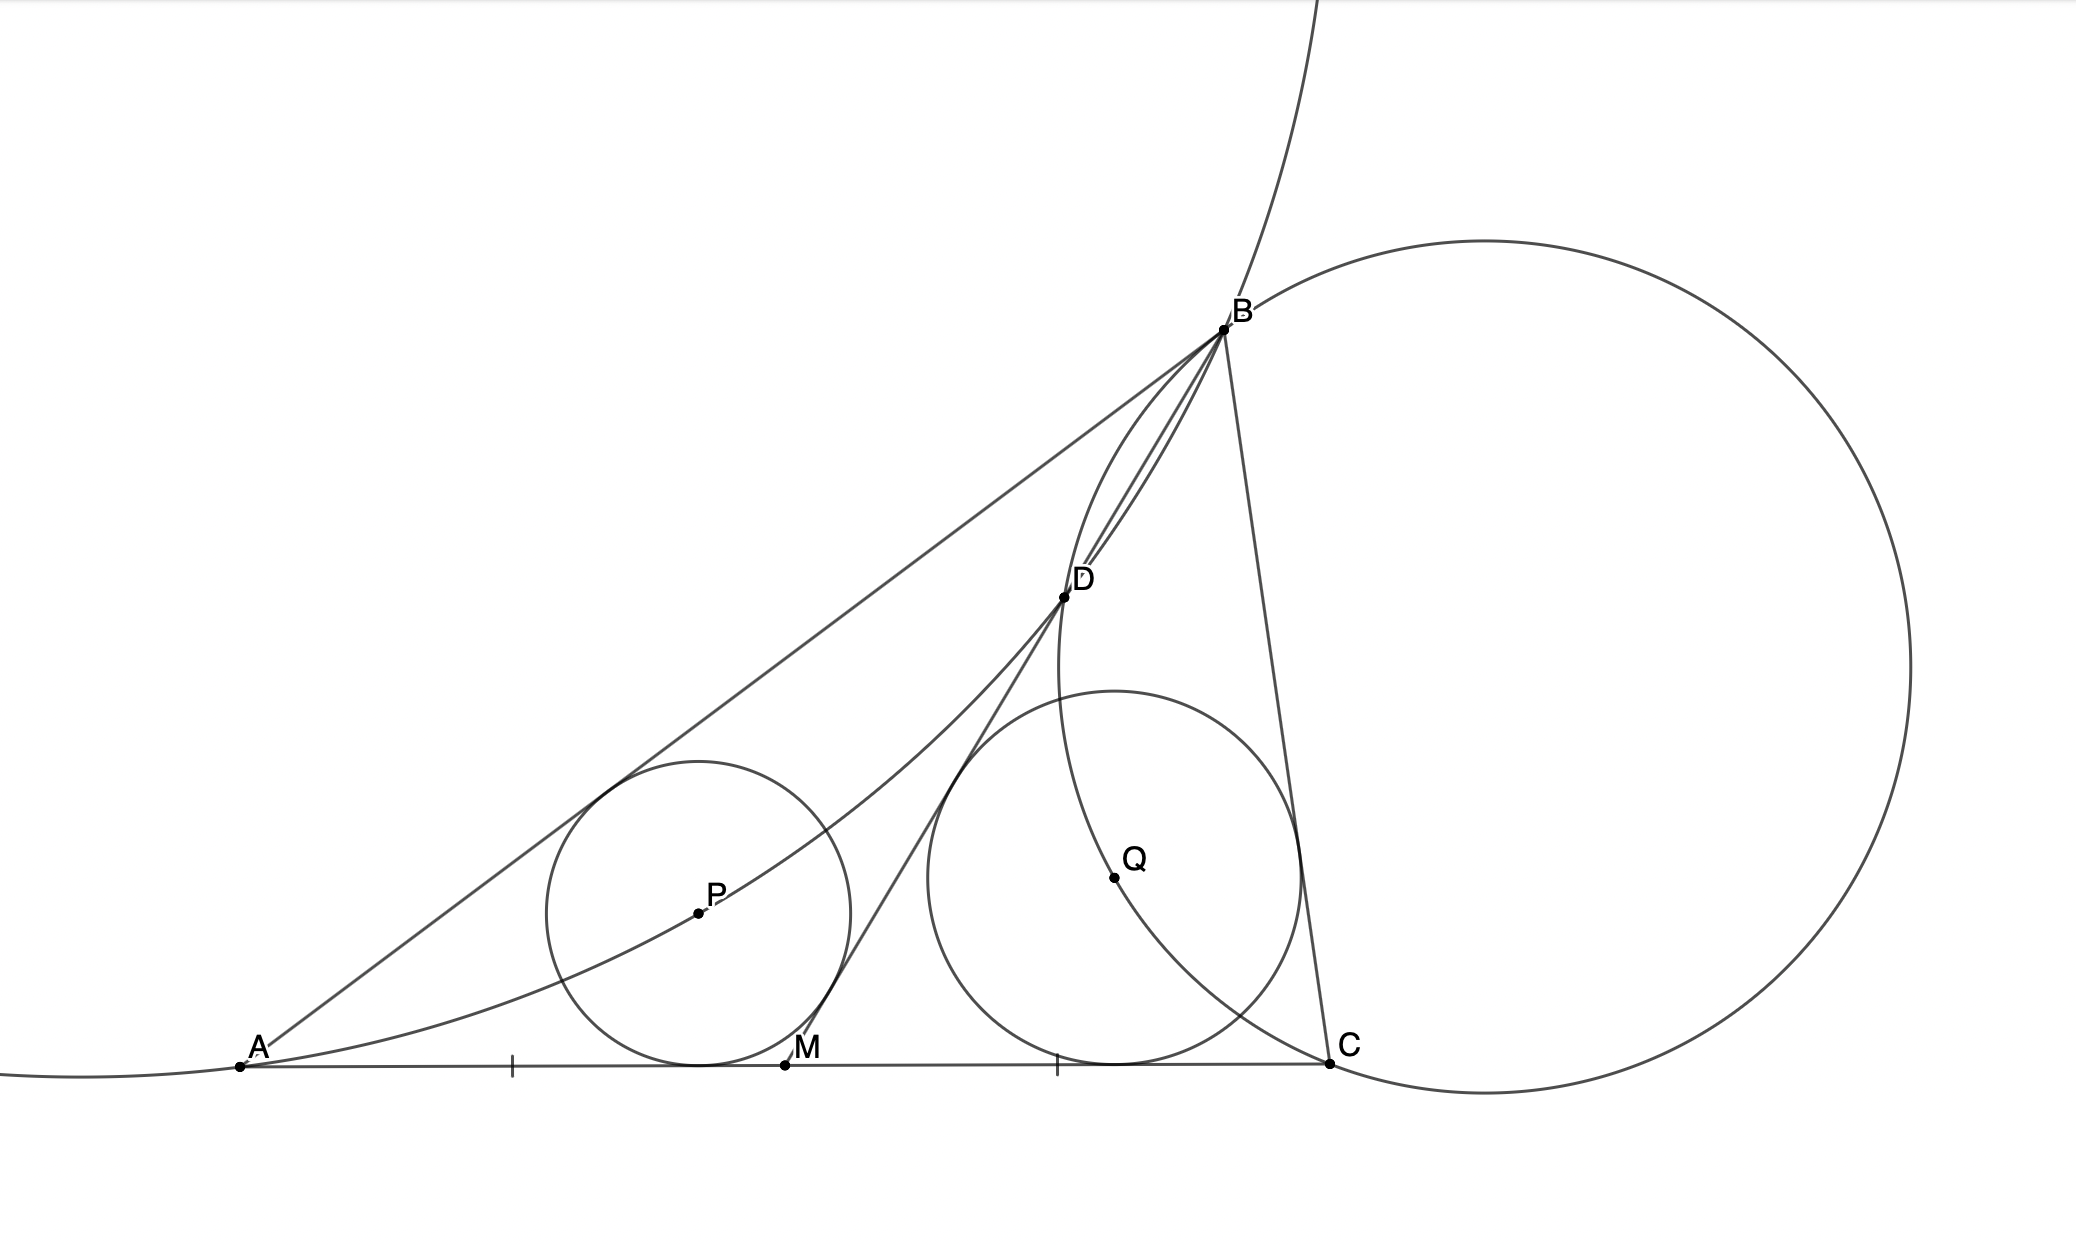
\includegraphics[width=1\linewidth]{ЭлМШ 2025-2026//III блок//10//Тренировки//II//Решения/9.5.png}
    \caption{Enter Caption}
    \label{fig:placeholder}
\end{figure}
%Москва 2018